\subsection{Levitation region}
\label{subsec:levitation_region}

From the analysis performed in Section \ref{subsec:force_analysis}, we can derive the levitation region of the system in which it's possible to maintain the ball in a levitated state provided that the force from the upper coil is greater than the gravitational force acting on the ball.

\begin{figure}[H]
    \centering
    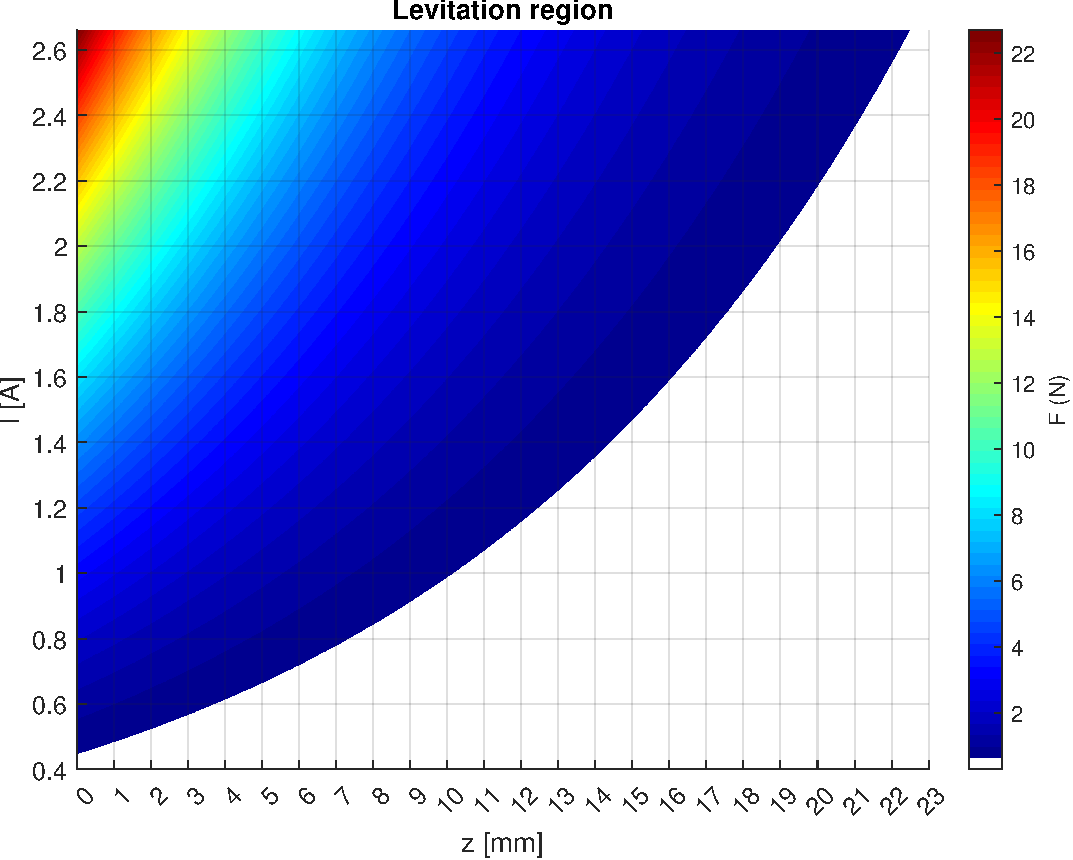
\includegraphics[width=0.7\textwidth]{./img/MATLAB/analysis/levitation_region.pdf}
    \caption{Levitation Region}
    \label{fig:levitation_region}
\end{figure}

From Figure \ref{fig:levitation_region}, it's also possible to see that the maximum distance from the upper coils before the ball falls is $z_{max} = 22.97 [mm]$ at values of the current equal to $I_{max} = 2.66 [A]$.